\section{Praxis}

\begin{frame}{Towel-Day!}
	\begin{center}
		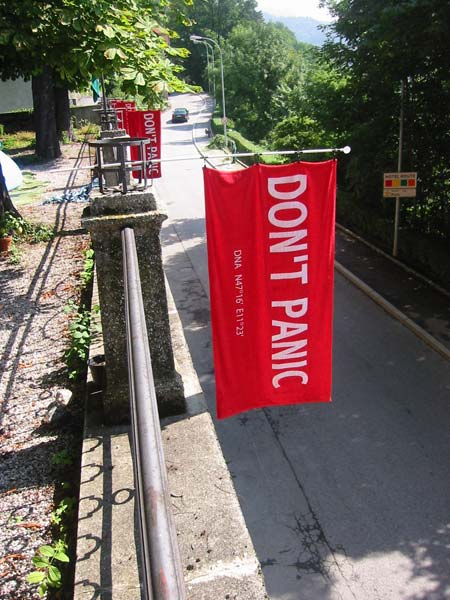
\includegraphics[height=0.8\textheight]{images/Towelday-Innsbruck.jpg}
	\end{center}
	
	\scriptsize
	\raisebox{4em}
	{
		Quelle: Wikimedia Commons
		CC-BY-SA 3.0 Beny Shlevich
	}
\end{frame}

\begin{frame}[fragile]{Praxis!}
	\begin{itemize}
		\item Aufgabe 1: Titel
		\item Aufgabe 2: Noch ein Titel
	\end{itemize}
	\ \\
	\ \\
	\large{\url{https://github.com/kit-cpp-workshop/workshop-ss12-04}} \\
	\ \\
	Aufgabenbeschreibungen und Hinweise: Siehe \verb|README.md|

\end{frame}
